% Chapter Template

\chapter{Ensayos y resultados} % Main chapter title

\label{Chapter4} % Change X to a consecutive number; for referencing this chapter elsewhere, use \ref{ChapterX}

En este capítulo se explica cómo se hicieron los ensayos y qué resultados se obtuvieron.
%----------------------------------------------------------------------------------------
%	SECTION 1
%----------------------------------------------------------------------------------------

\section{Banco de pruebas}
\label{sec:entornos}

Se utilizaron 3 entornos para llevar a cabo el desarrollo y las consecuentes pruebas del sistema. A nivel de \textit{software} se administraron utilizando un repositorio en la nube y manteniendo 3 ramas individuales de código, una para cada entorno. A nivel de \textit{hardware} se fue escalando entre entornos a medida que se avanzaba en el desarrollo y las pruebas.

Los entornos se denominaron de la siguiente manera:
\begin{itemize}
\item dev: para referirse a \textit{development} o desarrollo.
\item test: para referirse a \textit{testing} o pruebas.
\item prod: para referirse a \textit{production} o producción.
\end{itemize}

En la figura \ref{fig:entornos} se puede observar cada entorno y las tareas realizadas en cada uno.

\begin{figure}[H]
	\centering
	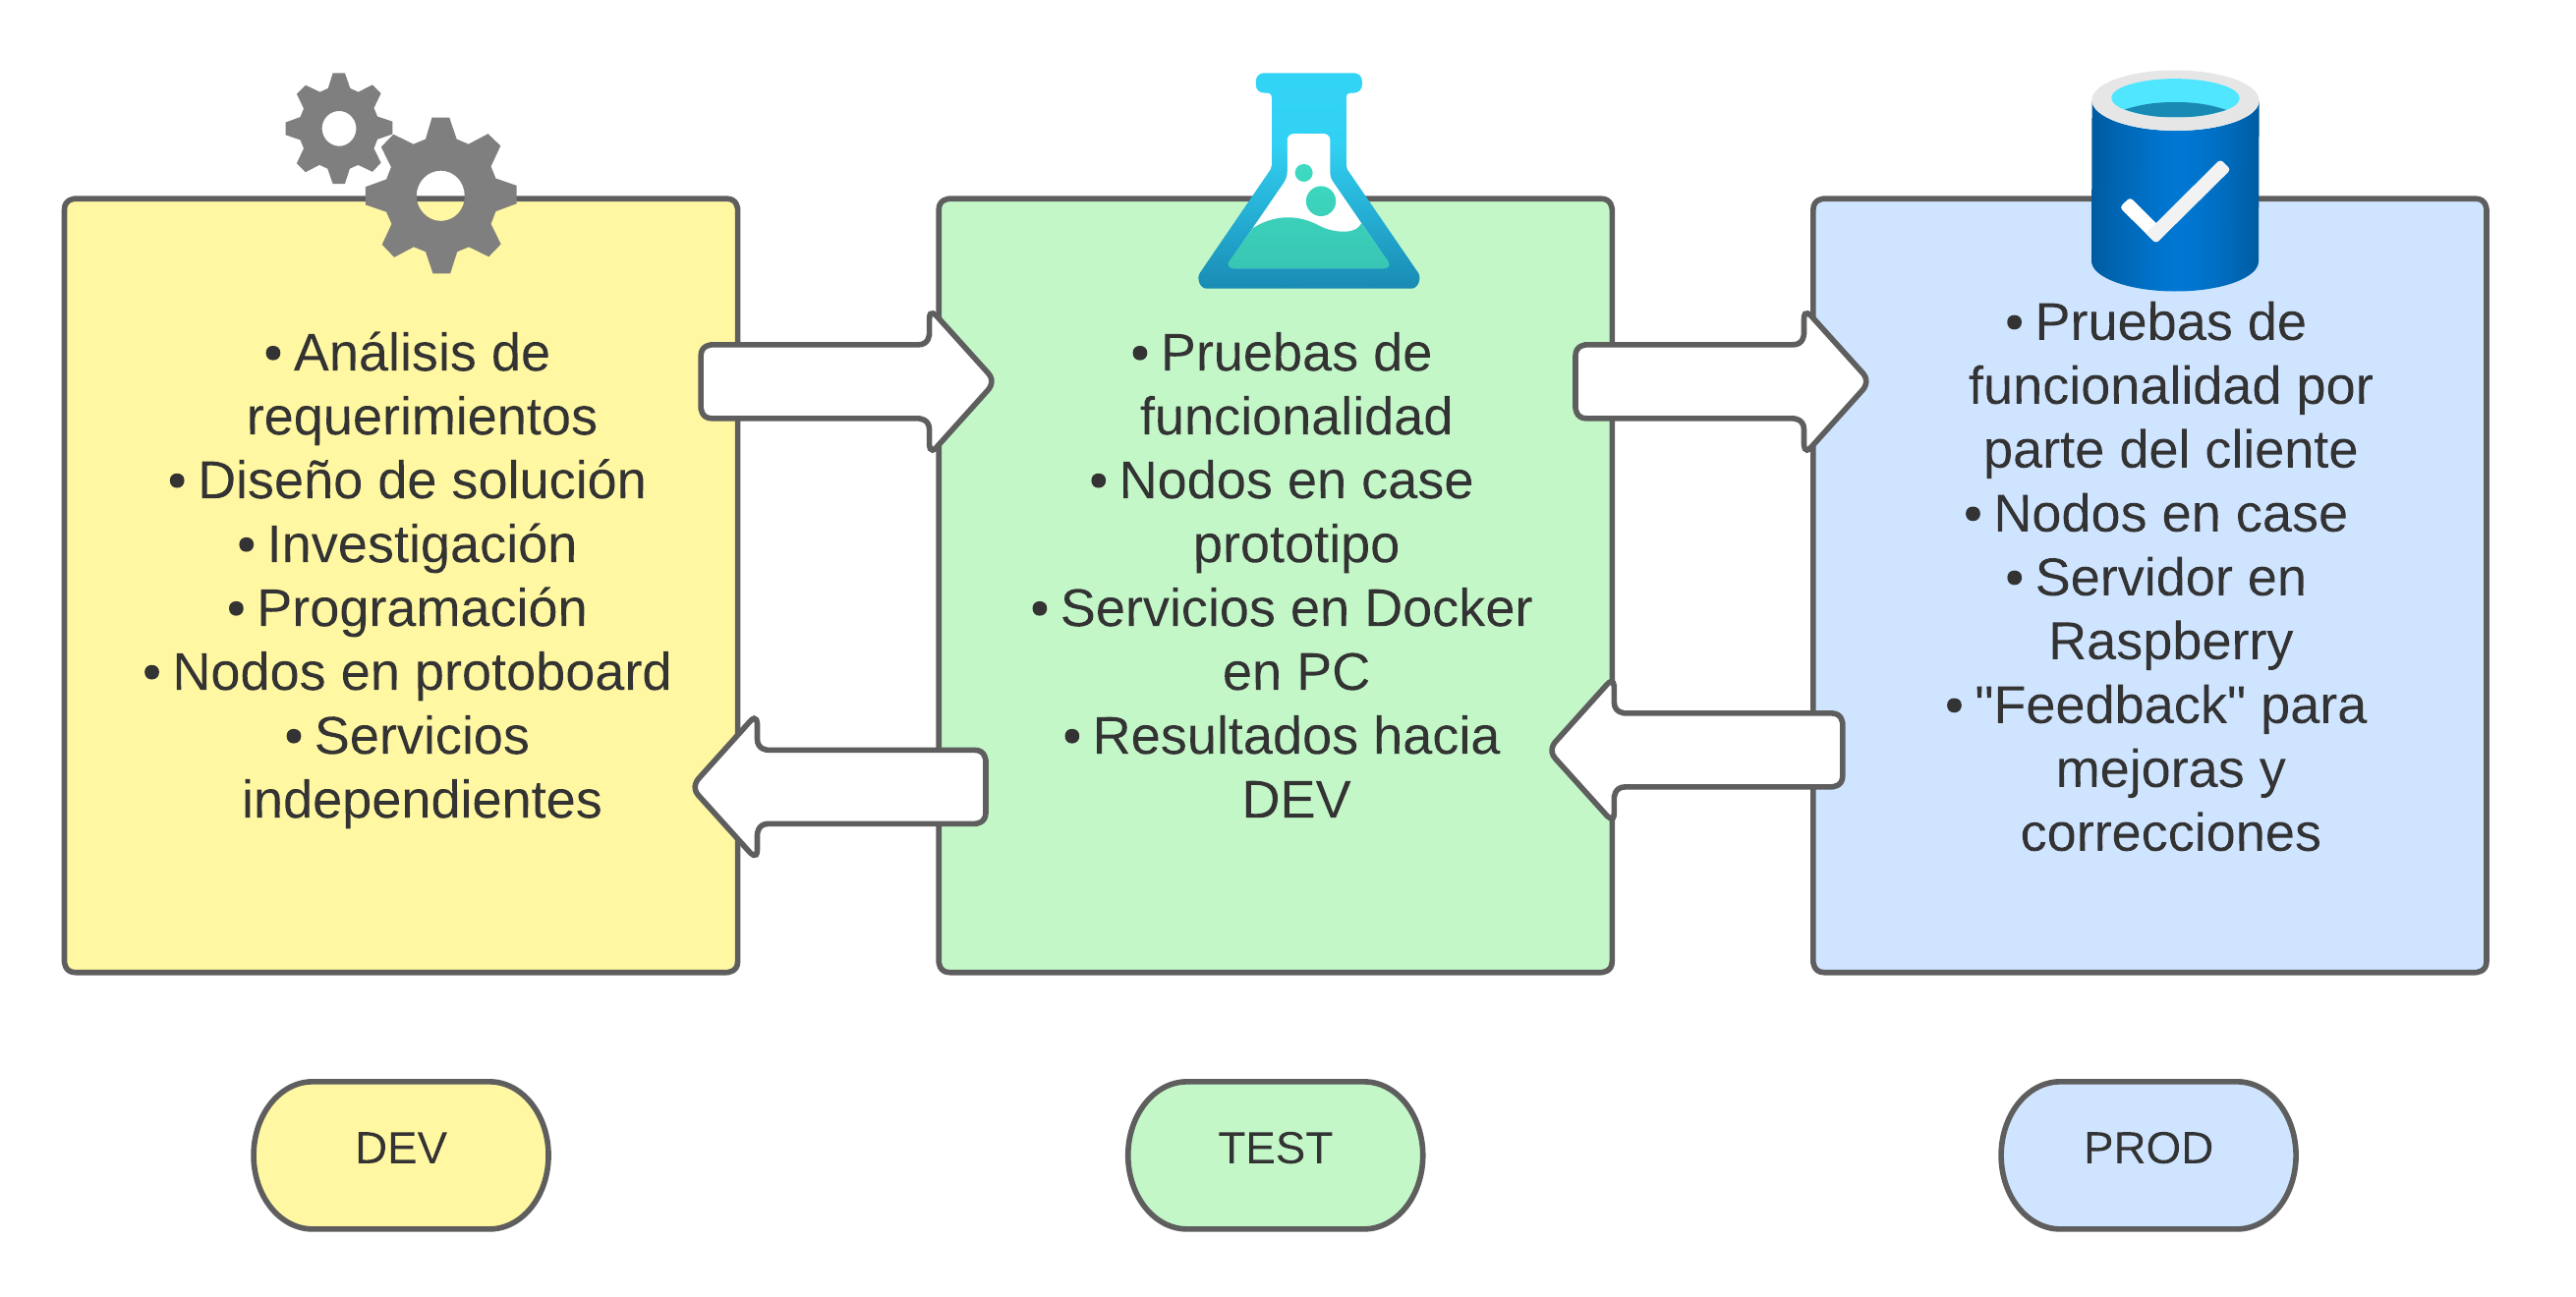
\includegraphics[scale=.15]{./Figures/diagrama-entornos.png}
	\caption{Entornos de desarrollo y pruebas del sistema.}
	\label{fig:entornos}
\end{figure}

\section{Ensayos sobre la API}
\label{sec:ensayos-api}

Para realizar las pruebas en las comunicaciones HTTP y validar la funcionalidad de la API de backend y la API Messenger, se utilizó la herramienta de prueba de API llamada Insomnia \cite{insomnia}, la cual permite hacer solicitudes utilizando los métodos HTTP.

Se creó la estructura de \textit{endpoints} del sistema separadas en carpetas y archivos según módulos o funcionalidad y se declararon los diferentes entornos de prueba (\textit{dev, test y prod}) descritos en la sección anterior. 

Se realizaron diversas pruebas como: la autenticación de usuario, la validación de parámetros de solicitud, el manejo de errores, las respuestas del servidor, la manipulación de datos en la base de datos y la integración de servicios de terceros, entre otras.

En las figuras \ref{fig:insomnia-carpetas} se muestra un ejemplo de la estructura de carpetas utilizadas y sus rutas, se pueden ver los métodos HTTP y el entorno utilizado, en este caso, \textit{dev localhost}.

\begin{figure}[H]
	\centering
	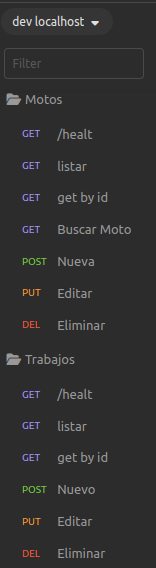
\includegraphics[scale=.60]{./Figures/insomnia-carpetas3.png}
	\caption{Estructura de carpetas y archivos en Insomnia.}
	\label{fig:insomnia-carpetas}
\end{figure}
  
En la figura \ref{fig:insomnia-request-1} se representa un ejemplo de una petición HTTP GET a la ruta para filtrar órdenes de trabajo.

\begin{figure}[H]
	\centering
	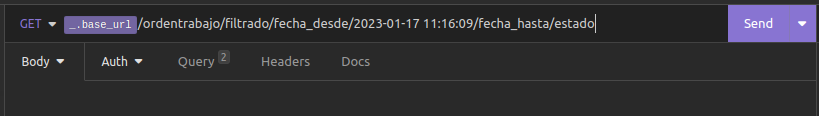
\includegraphics[width=\textwidth]{./Figures/insomnia-request-1.png}
	\caption{Petición HTTP GET en Insomnia.}
	\label{fig:insomnia-request-1}
\end{figure}

El parámetro \textit{base url} es una variable de entorno que trae la ruta base según el entorno en que se está trabajando, en este caso el entorno es \textit{dev localhost} y la variable \textit{http://localhost:3001}. Se observa la ruta y los parámetros en la URL. Se pueden añadir el \textit{body} y \textit{header} de la petición así como también el \textit{token} de autenticación.

En la figura \ref{fig:insomnia-request-2} se imprime la respuesta a la petición, dónde se indica el código de \textit{status} HTTP, en este caso 200, el tiempo de respuesta en milisegundos y el tamaño de la respuesta en \textit{Kilobytes}. En la pestaña \textit{Preview} muestra el resultado de la petición en formato JSON y se pueden ver en las siguiente pestañas el \textit{header, cookies y timeline} de la respuesta. 

\begin{figure}[H]
	\centering
	\includegraphics[scale=.65]{./Figures/insomnia-request-2.png}
	\caption{Respuesta de una petición en Insomnia.}
	\label{fig:insomnia-request-2}
\end{figure}


\section{Ensayos sobre el sistema}
\label{sec:ensayos-nodos}

Primeramente, durante la etapa de desarrollo \textit{dev} y \textit{test}, se fueron realizando pruebas a medida que se avanzaba en el desarrollo. Para esto se utilizaron placas de prototipo \textit{protoboard} para los nodos y se ejecutaron los sistemas en modo local utilizando Nodemon \cite{nodemon} y posteriormente Docker y Docker Compose, como se describe en la sección \ref{sec:entornos} del presente capítulo.

Luego de superadas las pruebas iniciales se procedió a las pruebas funcionales del sistema. Estas se realizaron sobre el sistema completo en ejecución, ya que todas las partes del sistema se comunican entre sí. 

Una vez que se conectaron todos los nodos y el servidor Raspberry Pi a la corriente eléctrica se realizaron las pruebas en el sistema web. Se realizó el recorrido completo del proceso de una orden de trabajo mientras se analizaba en paralelo las terminales de línea de comandos y la funcionalidad \textit{debug} del navegador.

Para comprobar el estado del servidor y acceder a los \textit{logs} de cada servicio se utilizó Portainer.

\subsection{Inicio del servidor}
\label{subsec:ensayoservidor}

Como primera medida se comprueba el estado del servidor y sus servicios. En la figura \ref{fig:ensayoportainer3} se puede observar el estado de los contenedores. La interfaz de Portainer además muestra el nombre, direcciónes IP, puertos, entre otros datos.

\begin{figure}[H]
	\centering
	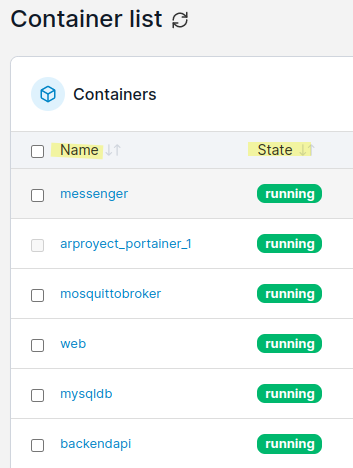
\includegraphics[scale=.70]{./Figures/ensayo-1/3.portainer2.png}
	\caption{Estado de contenedores.}
	\label{fig:ensayoportainer3}
\end{figure}

Se ingresa a los \textit{logs} del servicio de la API backend para verificar su funcionamiento.  En la figura \ref{fig:ensayoportainerlogapi} se observan los registros del \textit{log} donde resaltado con amarillo se puede observar la ejecución del log con Nodemon, el mensaje de conexión correcta al \textit{broker} MQTT, la suscripción a todos los tópicos y la conexión correcta a la base de datos.

En color verde se resaltan 3 líneas similares. Cada una de estas líneas corresponde a cada nodo que envió un mensaje de confirmación a la API, de esta manera se comprueba que los 3 nodos se conectaron correctamente al \textit{broker} MQTT.

\begin{figure}[H]
	\centering
	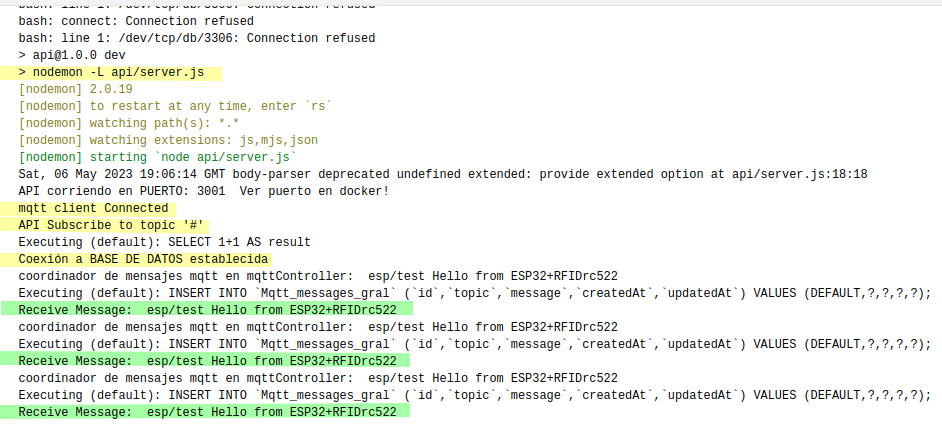
\includegraphics[scale=.90]{./Figures/ensayo-1/4.portainer-log-api.png}
	\caption{Estado de contenedores.}
	\label{fig:ensayoportainerlogapi}
\end{figure} 

\subsection{Carga de nueva órden de trabajo}
\label{subsec:ensayonuevaorden}

Inicio del proceso para el ingreso de una nueva orden de trabajo.

En la figura \ref{fig:ensayonueva1-1} se puede ver en detalle la sección donde se activa la función observador de Ionic para luego pasar la tarjeta por el nodo \textit{mostrador}. Una vez que se pasa la tarjeta por el lector aparecé el número de tarjeta que, para este ejemplo, está resaltado en color amarillo.

\begin{figure}[H]
	\centering
	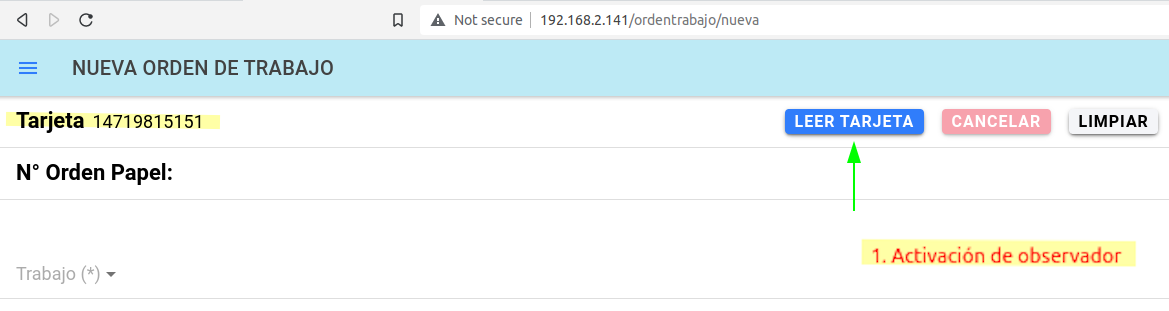
\includegraphics[width=\textwidth]{./Figures/ensayo-1/5.nueva-1.png}
	\caption{Interfaz para carga de nueva orden de trabajo.}
	\label{fig:ensayonueva1-1}
\end{figure}

En la figura \ref{fig:ensayonueva1-2} se presenta la sección \textit{debug} del navegador donde se ven los mensajes de impresión en consola para hacer análisis del sistema.

\begin{figure}[H]
	\centering
	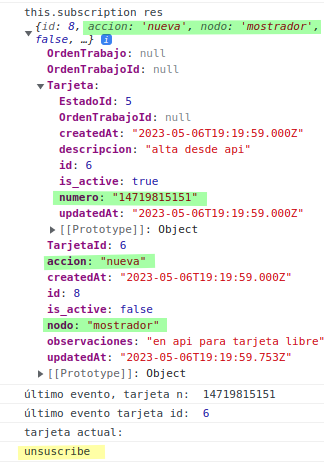
\includegraphics[scale=.90]{./Figures/ensayo-1/5.nueva-2.png}
	\caption{Sección \textit{debub} del navegador.}
	\label{fig:ensayonueva1-2}
\end{figure}

Se puede confirmar que la suscripción del observador se realizó correctamente cuando se hizo clic en ``LEER TARJETA``. Después se pasa la tarjeta RFID por el lector. 

En verde se resaltan los datos de la tarjeta leída. Como datos importantes se muestra:

\begin{enumerate}
\item acción = \textit{nueva}.
\item nodo = \textit{mostrador}.
\item número = 14719815151.
\end{enumerate}

Por último se imprime el mensaje \textit{unsuscribe}, el cual se resaltó en color amarillo,  este indica que la finalización del observador se realizó con éxito una vez concluida la lectura de la tarjeta. Esto es importante ya que el observador ocupa memoria en el sistema y genera tráfico de red. 

A continuación, en la figura \ref{fig:ensayo-nueva-logs} se muestra el log de la API backend. 

\begin{figure}[H]
	\centering
	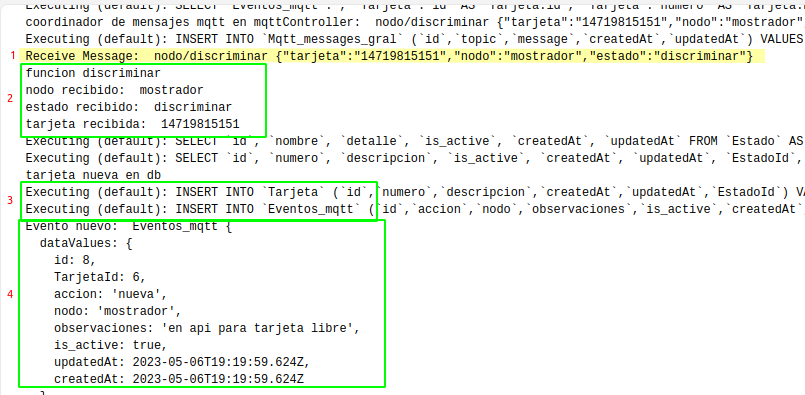
\includegraphics[scale=.95]{./Figures/ensayo-1/6.nueva-logs-1.png}
	\caption{Log API backend.}
	\label{fig:ensayo-nueva-logs}
\end{figure}

A fines de poder explicar mejor el registro se enumeraron los puntos importantes a la izquierda en la figura, los mismos se detallan a continuación:

\begin{enumerate}
\item \textit{Receive Message} se refiere a la recepción del mensaje por MQTT en la API. Se detalla el tópico \textit{nodo/discriminar} que indica que el mensaje proviene de un nodo y que la acción a ejecutar es discriminar, la cual se verifica en el código fuente por medio de funciones condicionales. El cuerpo del mensaje en formato JSON indica  el número de la tarjeta, el nombre del nodo, en este caso \textit{mostrador} y el \textit{estado} que indica que acción se debe tomar.

\item Dentro del recuadro resaltado en verde están los datos anteriormente detallados, los cuales se imprimen en el \textit{log} para una mejor lectura.

\item En este punto se muestran las funciones de insertar campos en la base de datos dentro de las tablas \textit{Tarjeta} y \textit{Eventos mqtt}. En la tabla \textit{Tarjeta} se registran los datos de la misma ya que no existe previamente en la base de datos, su estado será \textit{libre} hasta que se confirme el ingreso de la orden. En la tabla \textit{Eventos mqtt} se registra que ingresó una tarjeta libre, mediante este registro el observador de Ionic tomará los datos de la tarjeta para insertarlos en el formulario para la nueva orden de trabajo.

\item En este recuadro se muestra la información detallada que se ingresó en la tabla \textit{Eventos mqtt}, se puede observar que tiene la relación a el ID de la tarjeta, la acción \textit{nueva} y el nodo \textit{mostrador}.
\end{enumerate}

Los próximos pasos que se ejecutan son los de agregar los datos del cliente y la moto para la orden de trabajo, verificando el correcto funcionamiento de los formularios correspondientes. Además se completa el campo \textit{detalle} y \textit{costos}.

Una vez completado el formulario se hace clic en \textit{Guardar y Limpiar} y se confirma la operación.

En la figura \ref{fig:ensayonueva10} se imprimen los registros en la consola del navegador web.

\begin{figure}[H]
	\centering
	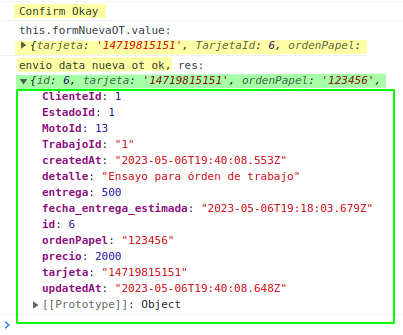
\includegraphics[scale=1.1]{./Figures/ensayo-1/10.nueva-res.png}
	\caption{Consola del navegador web.}
	\label{fig:ensayonueva10}
\end{figure}

Resaltado en amarillo se muestra que luego de la confirmación se enviaron correctamente los datos en formato JSON. Luego, en verde, los datos recibidos desde la API, lo cual indica que se procesó la petición correctamente. En la respuesta se imprimen los datos que fueron cargados en la base de datos, los datos del modelo orden de trabajo y los IDs de los modelos que tienen relación con este registro.

En la figura \ref{fig:ensayonueva10-2} se puede observar el \textit{log} de la API.

\begin{figure}[H]
	\centering
	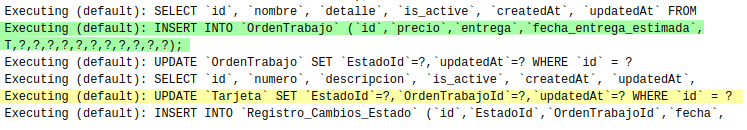
\includegraphics[width=\textwidth, height=4cm]{./Figures/ensayo-1/10.nueva-api-log.png}
	\caption{\textit{Logs} de la API.}
	\label{fig:ensayonueva10-2}
\end{figure}

Se resalta en verde el proceso que inserta los registros en la base de datos en el modelo ``OrdenTrabajo``. En amarillo, se resalta el proceso que actualiza los datos de la tarjeta, principalmente se actualiza su estado a ``en uso`` y se la relaciona a la ` de trabajo creada.

Finalmente se navega en la aplicación web hacia la pestaña ``Listado`` donde se puede verificar la orden creada. En la figura \ref{fig:ensayolistado} se muestra, resaltado en amarillo, el nuevo registro. En esta pantalla se actualiza el estado de las ordenes automáticamente.

\begin{figure}[H]
	\centering
	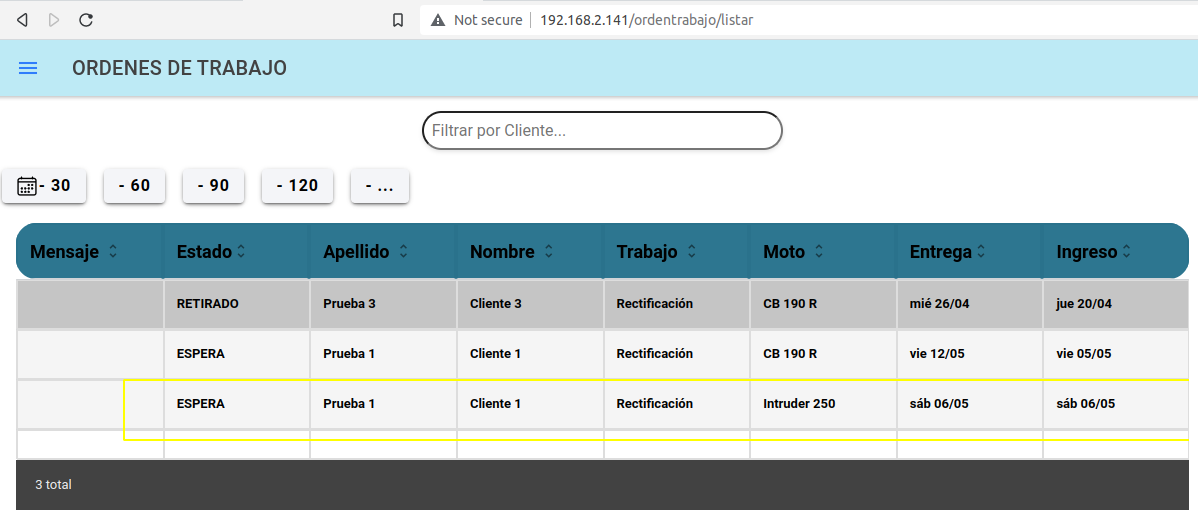
\includegraphics[width=\textwidth]{./Figures/ensayo-1/11.listado.png}
	\caption{Listado de órdenes de trabajo.}
	\label{fig:ensayolistado}
\end{figure}

\subsection{Cambio a estado proceso}
\label{subsec:ensayoaproceso}

En esta sección verificamos el cambio de estado de la orden de trabajo creada previamente. Se asigna el estado ``en proceso``.

Se pasa la tarjeta RFID, correspondiente a la orden de trabajo creada en la sección previa, por el nodo ``proceso`` y se verifican los resultados en el log de la API backend.

En la figura \ref{fig:cambioestado-api-log} se observan los resultados del \textit{log}.

\begin{figure}[H]
	\centering
	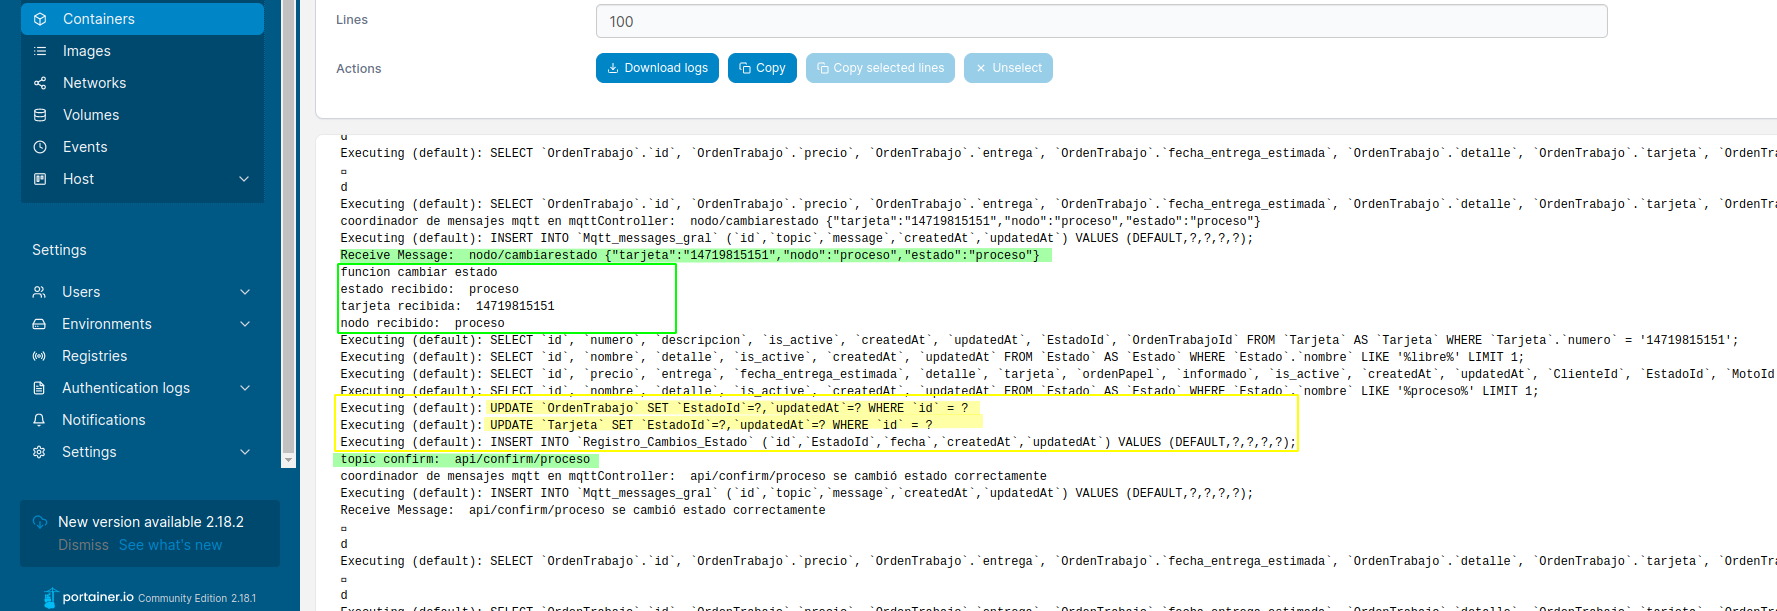
\includegraphics[width=\textwidth, height=6cm]{./Figures/ensayo-1/12.cambioestado-api-log.png}
	\caption{\textit{Logs} de API en cambio de estado.}
	\label{fig:cambioestado-api-log}
\end{figure}

En color verde, se resaltan los registros referentes a la comunicación MQTT, en la primer línea resaltada corresponde a la recepción del mensaje indicada con el mensaje \textit{Receive Message} y los detalles del mismo donde indica el número de tarjeta, el nodo emisor y el estado o acción a ejecutar.

Luego, se resaltan en amarillo las líneas que indican los procesos sobre la base de datos, en este caso son dos actualizaciones o \textit{UPDATES}, una sobre la tabla ``OrdenTrabajo`` y la otra sobre la tabla ``Tarjeta``, en ambas se actualiza el estado utilizando al relación con la tabla ``Estado``.

Por último se resalta en verde la línea que indica el envío de un mensaje de confirmación MQTT al nodo emisor para que se realice el alerta sonora correspondiente.

Se navega a la pantalla ``Listado`` de la aplicación \textit{web} y se verifica el cambio de estado. En la figura \ref{fig:ensayolistadoweb} se observa el resultado. La orden ha sido actualizada a estado ``PROCESO`` y cambió el color de la fila correspondiente.

\begin{figure}[H]
	\centering
	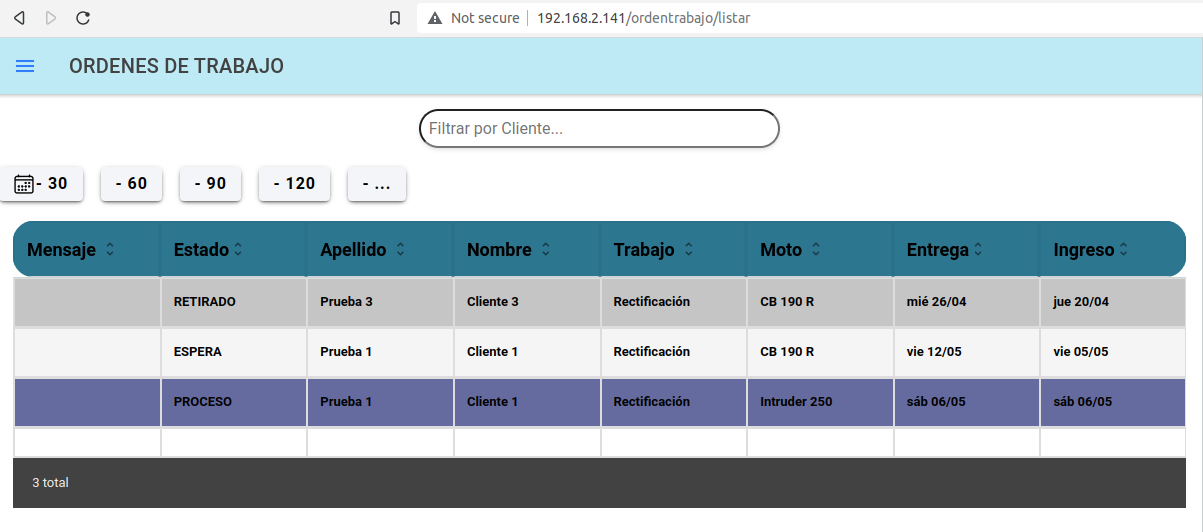
\includegraphics[width=\textwidth]{./Figures/ensayo-1/12.cambioestado-listado.png}
	\caption{Listado de órdenes de trabajo}
	\label{fig:ensayolistadoweb}
\end{figure}

\subsection{Cambio a estado finalizado}
\label{subsec:ensayoafinalizado}

En esta sección se verifica el cambio de estado de la orden de trabajo al estado ``finalizado``.

Siguiendo el procedimiento, se pasa la tarjeta RFID correspondiente por el nodo ``finalizado`` y se analizan los resultados en el log de la API backend.

En la figura \ref{fig:ensayofinalizadoapi} se muestra el l\textit{log}.

\begin{figure}[H]
	\centering
	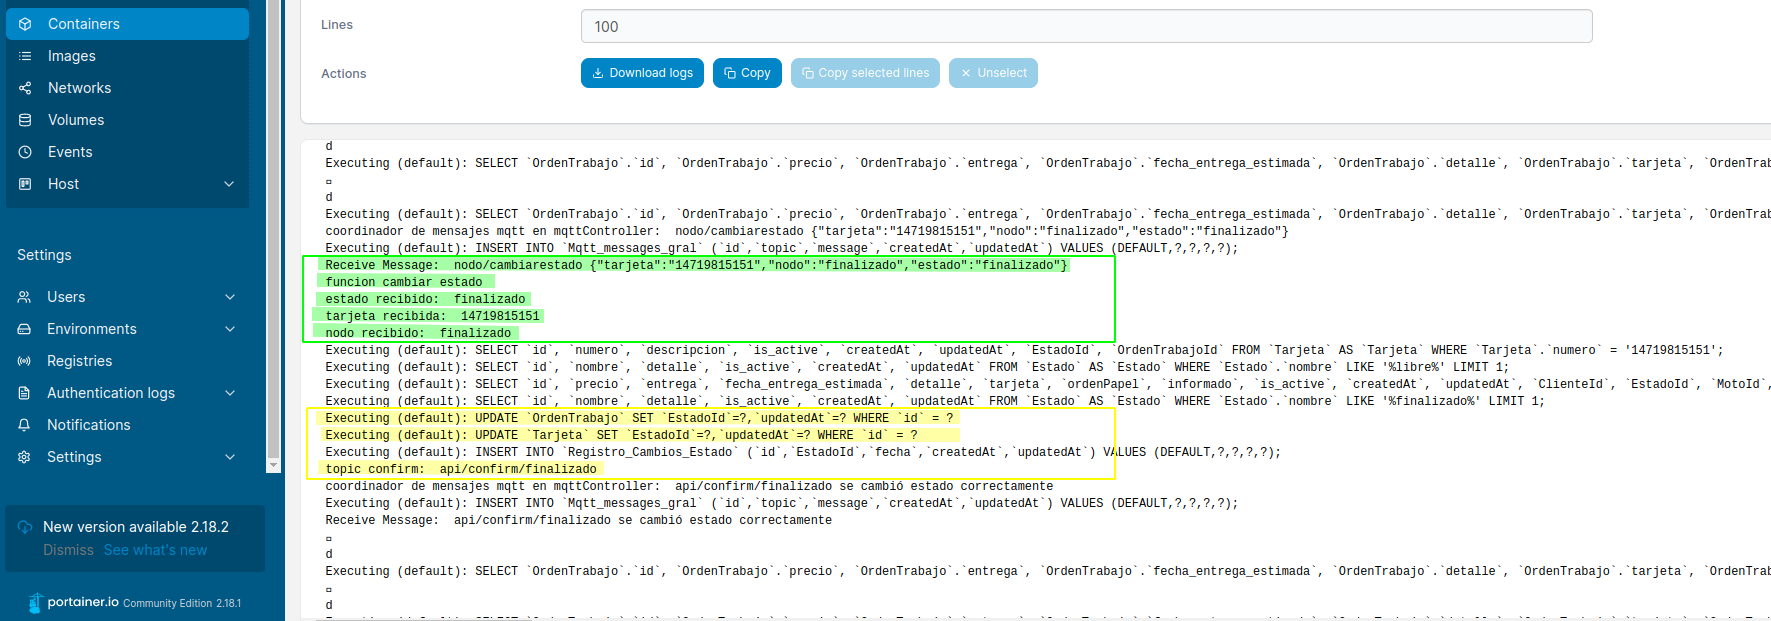
\includegraphics[width=\textwidth, height=6cm]{./Figures/ensayo-1/13.finalizado-api-logs.png}
	\caption{\textit{Logs} de Api en finalizado.}
	\label{fig:ensayofinalizadoapi}
\end{figure}

Se resalta en verde la confirmación de la recepción del mensaje MQTT en el tópico ``nodo/cambiarestado``, con el cuerpo del mensaje en formato JSON. En este caso el estado es ``finalizado``, lo que indica a que estado debe cambiar la orden de trabajo.

En amarillo se resaltan los procesos que se realizaron sobre la base de datos, nuevamente se ejecuta un \textit{UPDATE} en las tablas ``OrdenTrabajo`` y ``Tarjeta`` en el campo ``EstadoId`` que es la clave foránea de la tabla ``Estado``.

Por último se envía la confirmación por MQTT al nodo receptor, en este caso el nodo ``finalizado``.

En la figura \ref{fig:ensayofinalizadolistado} se muestra la aplicación \textit{web} en la sección ``Listado``, se puede confirmar el cambio de estado correspondiente en la tabla, el cambio de color de la fila y la correcta visualización del botón con el logo de la aplicación de mensajería.

\begin{figure}[H]
	\centering
	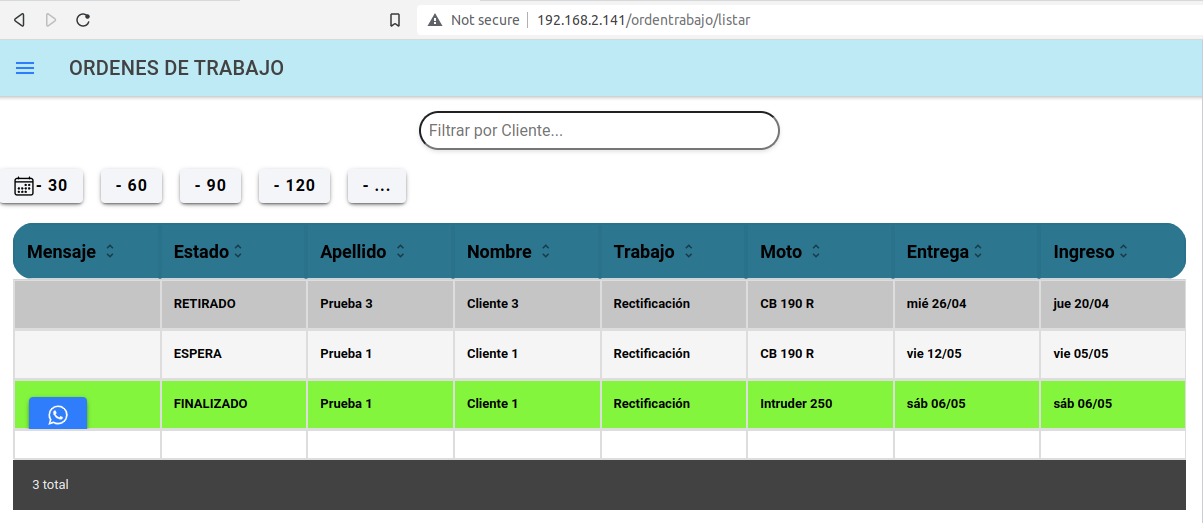
\includegraphics[width=\textwidth]{./Figures/ensayo-1/14.finalizado-listado.png}
	\caption{Listado de órdenes de trabajo.}
	\label{fig:ensayofinalizadolistado}
\end{figure}


\subsection{Envío de mensaje de texto}
\label{subsec:ensayomensaje}

Se verifica la autenticación al servicio de mensajería a través del código QR. 

En la aplicación \textit{web} se ingresa a la sección QR, primero se hace clic en ``Actualizar`` para verificar la función para renovar el código QR y luego se escanea el código con la cámara de un \textit{smartphone}.

En la figura \ref{fig:ensayomensaje1} se observa el resultado de una correcta autenticación. Debido a que la API de mensajería utiliza una biblioteca del navegador Google Chrome, en el listado aparece este navegador como dispositivo vinculado.

\begin{figure}[H]
	\centering
	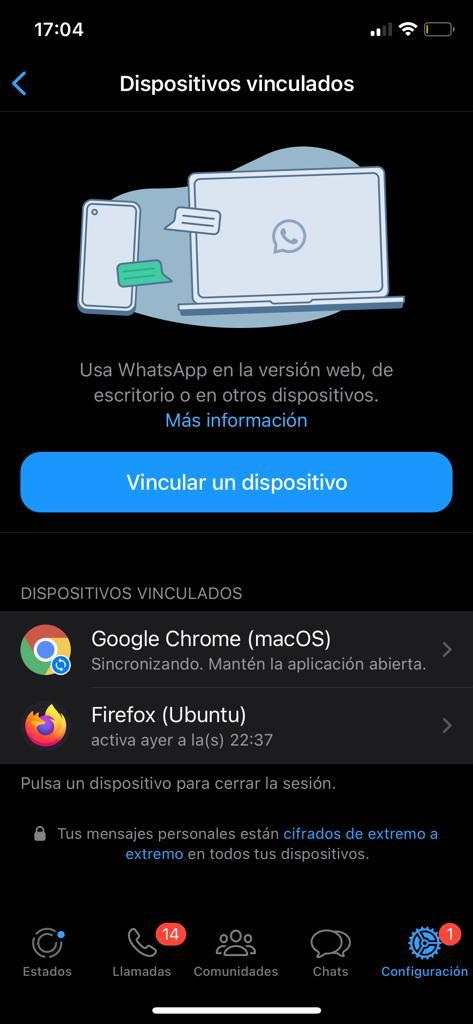
\includegraphics[scale=.30]{./Figures/ensayo-1/15.qr-api.jpeg}
	\caption{Vinculación a WhatsApp desde un \textit{Smartphone}}
	\label{fig:ensayomensaje1}
\end{figure}

En la figura \ref{fig:ensayomensajeapi} se puede observar el \textit{log} de la API Messenger donde indica, resaltado en amarillo, un primer \textit{logout} referente a la actualización del código QR realizada, luego se muestra el mensaje \textit{LOGIN SUCCESS} que indica que la autenticación se realizó con éxito.

\begin{figure}[H]
	\centering
	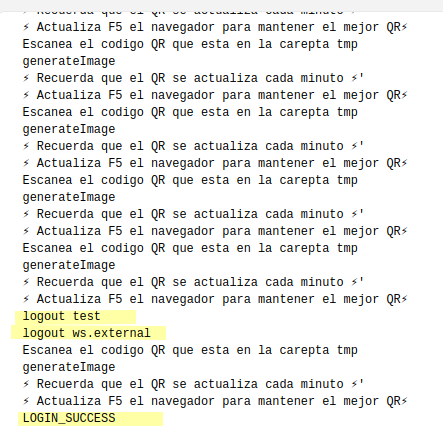
\includegraphics[scale=.99]{./Figures/ensayo-1/15-qr-api.png}
	\caption{\textit{Logs} de API Messenger.}
	\label{fig:ensayomensajeapi}
\end{figure}	

Siguiendo el flujo de la aplicación web, se confirma el mensaje para el envío. 

En la figura \ref{fig:ensayomensajewcel2} se muestra el mensaje recibido.

\begin{figure}[H]
	\centering
	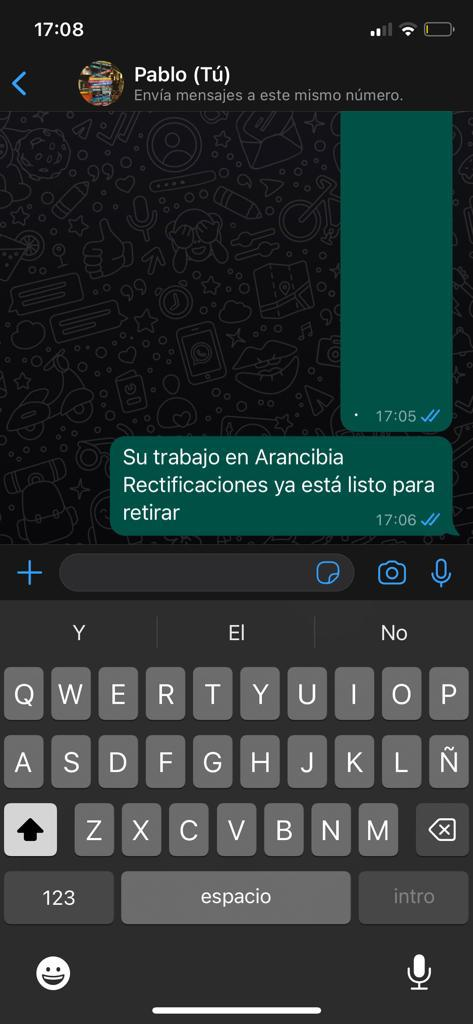
\includegraphics[scale=.30]{./Figures/ensayo-1/15.qr-api-1.jpeg}
	\caption{Mensaje de WhatsApp recibido}
	\label{fig:ensayomensajewcel2}
\end{figure}

En la figura \ref{fig:ensayomensajefinalizado} se puede confirmar el cambio de color a verde opaco de la fila correspondiente. Esto indica que el cliente ya fue informado respecto a su orden de trabajo.

\begin{figure}[H]
	\centering
	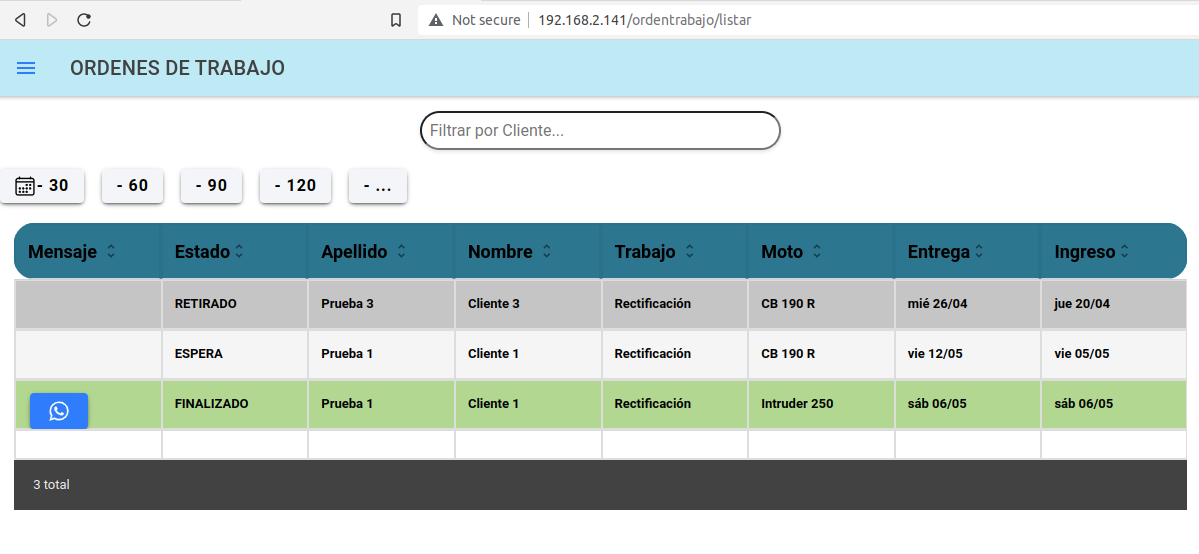
\includegraphics[width=\textwidth]{./Figures/ensayo-1/17.finalizado.png}
	\caption{Listado de órdenes de trabajo.}
	\label{fig:ensayomensajefinalizado}
\end{figure}

Se ensaya la funcionalidad de reenvio de mensaje. En este caso vuelve a mostrar un modal de confirmación de envío pero con el texto ``Reenviar Mensaje``. Se confirma el mensaje y se controla en el \textit{smartphone} la recepción. En la figura \ref{fig:ensayomensajecel2} se muestra el resultado.

\begin{figure}[H]
	\centering
	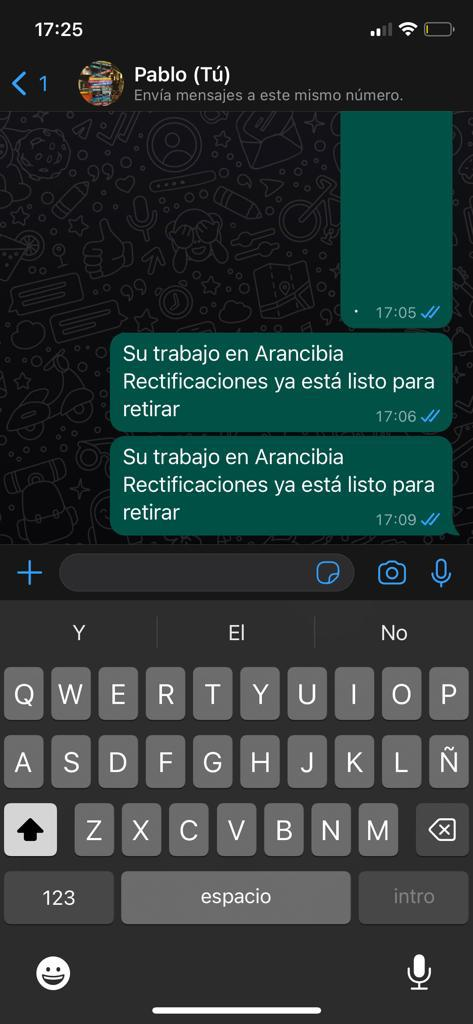
\includegraphics[scale=.30]{./Figures/ensayo-1/15.qr-api-2.jpeg}
	\caption{Mensaje de WhatsApp recibido}
	\label{fig:ensayomensajecel2}
\end{figure}

Por último se controla en la API backend el \textit{log} que indica si el cliente fue informado de la finalización de su orden de trabajo.

En la figura \ref{fig:ensayomensajeapilog} se resalta en amarillo la línea que confirma la actualización del campo ``informado`` en la tabla ``OrdenTrabajo``.

\begin{figure}[H]
	\centering
	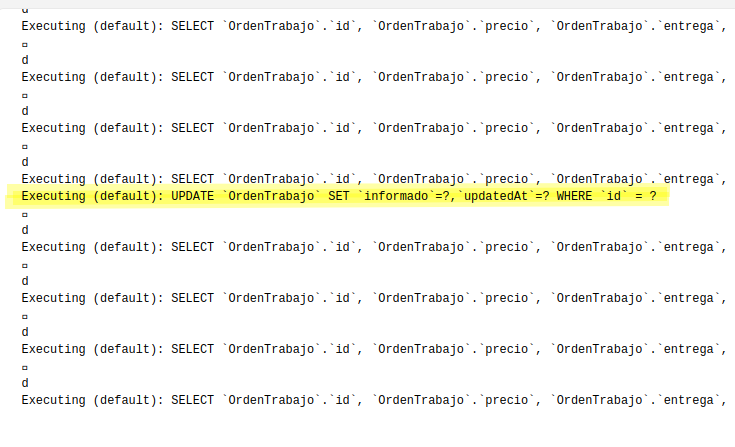
\includegraphics[width=\textwidth]{./Figures/ensayo-1/20.mensaje-api-log.png}
	\caption{\textit{log} de API backend.}
	\label{fig:ensayomensajeapilog}
\end{figure}


\subsection{Cambio a estado retirado}
\label{subsec:ensayoretiro}

La finalización del ciclo de estados de órdenes de trabajo se da cuando el cliente pasa a retirar su repuesto. En este caso el usuario del sistema debe ingresar a la sección ``Retirar`` en la aplicación \textit{web}, activar el modo escucha con el botón ``Leer Tarjeta`` y pasar la tarjeta RFID correspondiente por el nodo ``mostrador``.

En la figura \ref{fig:ensayoretirar-web-1} se muestra una parte de la interfaz para retirar una orden de trabajo donde se cargó automáticamente el número de tarjeta, luego de pasarla por el nodo lector, y se insertaron los datos del cliente.

\begin{figure}[H]
	\centering
	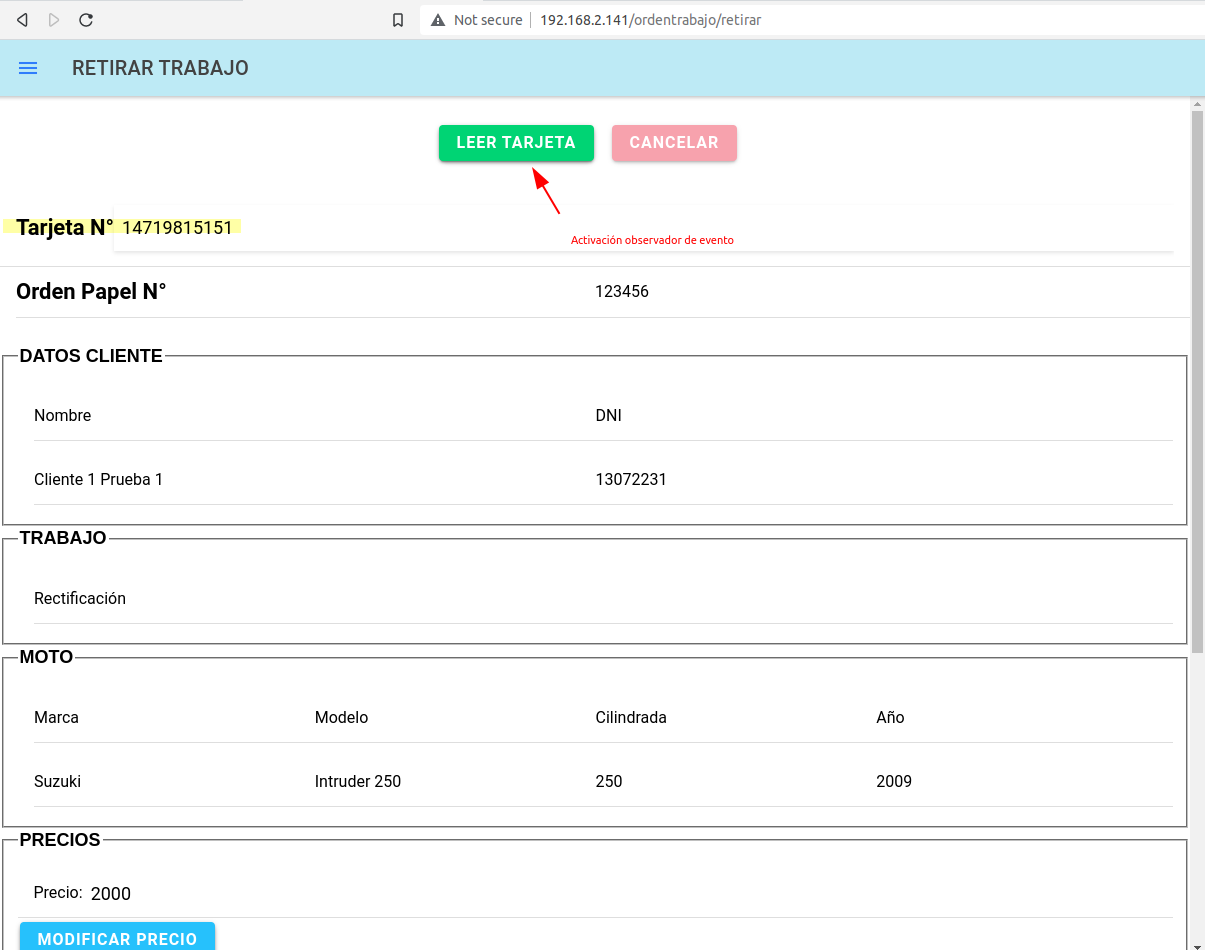
\includegraphics[width=\textwidth]{./Figures/ensayo-1/21.retirar-web-1.png}
	\caption{Interfaz para retirar orden de trabajo.}
	\label{fig:ensayoretirar-web-1}
\end{figure}

En la figura \ref{fig:ensayoretirar-web-2} se muestra la consola del navegador donde se observan los datos de la orden de trabajo recibidos desde la API, ya que cuando se pasa la tarjeta por el mostrador la API backend recibe y procesa la información y luego esta es leída por la aplicación \textit{web}. Resaltado en verde se observan todos los datos de la orden de trabajo y resaltado en celeste se pueden ver los datos de la tarjeta. estos datos son insertados en el formulario de retiro.

\begin{figure}[H]
	\centering
	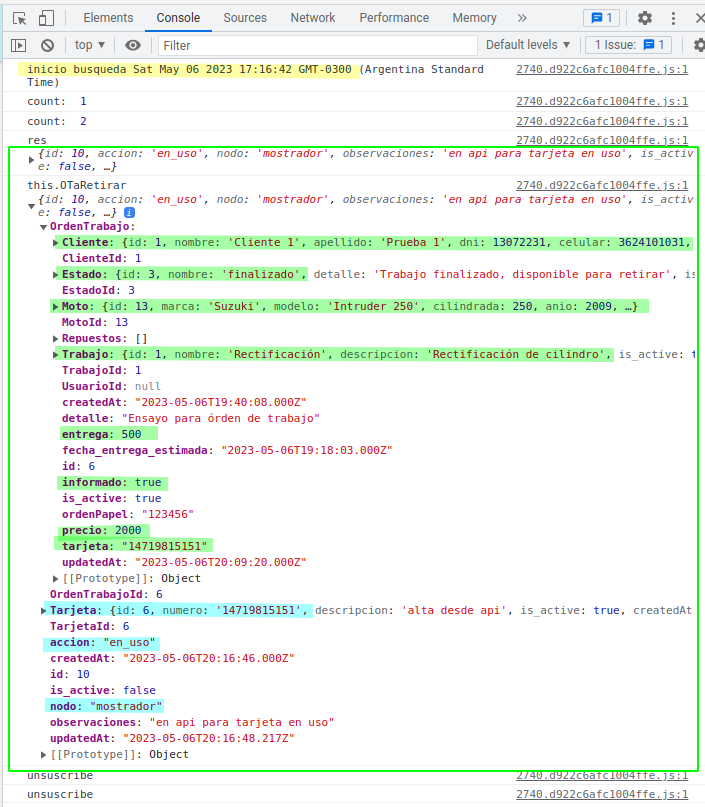
\includegraphics[width=\textwidth]{./Figures/ensayo-1/21.retirar-web-2.png}
	\caption{Consola de \textit{debug} del navegador.}
	\label{fig:ensayoretirar-web-2}
\end{figure}

En la figura \ref{fig:ensayoretirarapievento} se pueden observar los registros en el \textit{log} de la API backend. En verde están los datos correspondientes a la recepción del mensaje MQTT desde el nodo ``mostrador``. Se recibe el número de tarjeta y la acción ``discriminar``. Luego de procesar la información , se muestran en amarillo las líneas donde se confirma que se inserta en la base de datos el evento para que luego sea leído por la aplicación \textit{web} y se envía la respuesta por MQTT al nodo emisor, en este caso el nodo ``mostrador``.  

\begin{figure}[H]
	\centering
	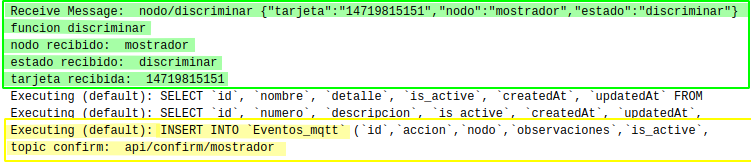
\includegraphics[width=\textwidth, height=5cm]{./Figures/ensayo-1/22.retirar-api-evento.png}
	\caption{\textit{Logs} de recepción MQTT en API backend.}
	\label{fig:ensayoretirarapievento}
\end{figure}

Luego que en la aplicación \textit{web} se insertaron los datos de la orden de trabajo, se confirma finalmente el retiro. En la figura \ref{fig:ensayoretirarconfirmacionapi} se ven, resaltados en amarillo, los registros en el \textit{log} de la API backend pertenecientes a la actualización de la tabla ``OrdenTrabajo`` y ``Tarjeta``. 
 
\begin{figure}[H]
	\centering
	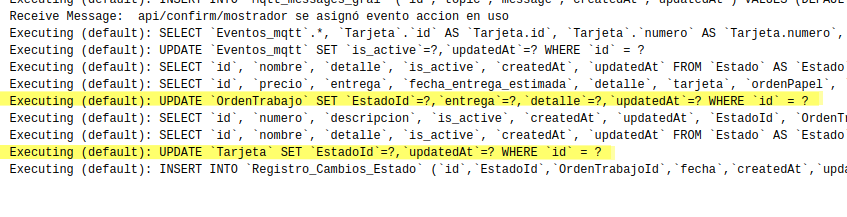
\includegraphics[width=\textwidth]{./Figures/ensayo-1/24.retirar-confirmacion-api.png}
	\caption{\textit{Logs} de confirmación de retiro en API backend.}
	\label{fig:ensayoretirarconfirmacionapi}
\end{figure}

De esta manera finaliza el ciclo de una orden de trabajo en el sistema. Se pudo observar en cada paso los resultados y \textit{logs} obtenidos y así asegurar el buen funcionamiento de los diferentes servicios desarrollados e implementados.




